\pdfminorversion=4
\documentclass[aspectratio=169]{beamer}

\mode<presentation>
{
  \usetheme{default}
  \usecolortheme{default}
  \usefonttheme{default}
  \setbeamertemplate{navigation symbols}{}
  \setbeamertemplate{caption}[numbered]
  \setbeamertemplate{footline}[frame number]  % or "page number"
  \setbeamercolor{frametitle}{fg=white}
  \setbeamercolor{footline}{fg=black}
} 

\usepackage[english]{babel}
\usepackage[utf8x]{inputenc}
\usepackage{tikz}
\usepackage{courier}
\usepackage{array}
\usepackage{bold-extra}
\usepackage{minted}
\usepackage[thicklines]{cancel}
\usepackage{fancyvrb}
\usepackage{tabto}

\xdefinecolor{dianablue}{rgb}{0.18,0.24,0.31}
\xdefinecolor{darkblue}{rgb}{0.1,0.1,0.7}
\xdefinecolor{darkgreen}{rgb}{0,0.5,0}
\xdefinecolor{darkgrey}{rgb}{0.35,0.35,0.35}
\xdefinecolor{darkorange}{rgb}{0.8,0.5,0}
\xdefinecolor{darkred}{rgb}{0.7,0,0}
\definecolor{darkgreen}{rgb}{0,0.6,0}
\definecolor{mauve}{rgb}{0.58,0,0.82}

\title[03-ecosystem]{The Numpy Ecosystem}
\author{Jim Pivarski}
\institute{Princeton University}
\date{November 15, 2018}

\usetikzlibrary{shapes.callouts}

\begin{document}

\logo{\pgfputat{\pgfxy(0.11, 7.4)}{\pgfbox[right,base]{\tikz{\filldraw[fill=dianablue, draw=none] (0 cm, 0 cm) rectangle (50 cm, 1 cm);}\mbox{\hspace{-8 cm}
\includegraphics[height=1 cm]{princeton-logo-long.png}\mbox{\hspace{0.25 cm}}}}}}

\begin{frame}
  \titlepage
\end{frame}

\logo{\pgfputat{\pgfxy(0.11, 7.4)}{\pgfbox[right,base]{\tikz{\filldraw[fill=dianablue, draw=none] (0 cm, 0 cm) rectangle (50 cm, 1 cm);}\mbox{\hspace{-8 cm}
\includegraphics[height=1 cm]{princeton-logo.png}\mbox{\hspace{0.25 cm}}}}}}

% Uncomment these lines for an automatically generated outline.
%\begin{frame}{Outline}
%  \tableofcontents
%\end{frame}

% START START START START START START START START START START START START START

\begin{frame}{The ecosystem: a vague word for a vague thing}
\vspace{0.27 cm}
\begin{columns}
\column{0.74\linewidth}
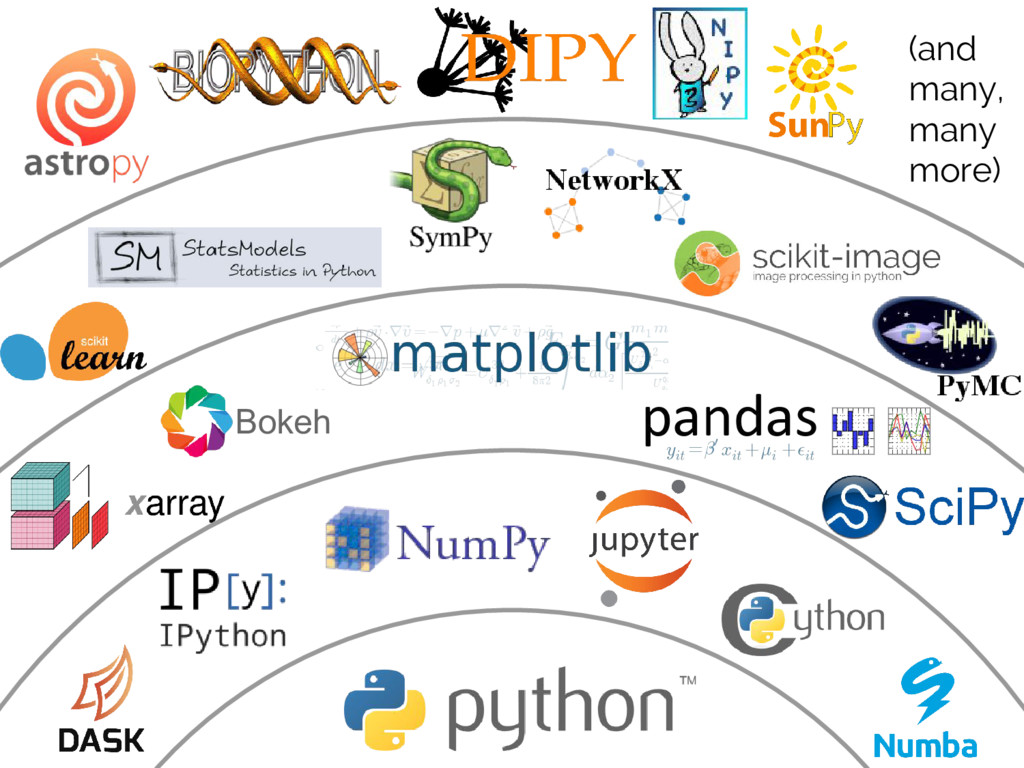
\includegraphics[width=\linewidth]{shells-5.png}
\end{columns}
\end{frame}

\begin{frame}{What we'll talk about this afternoon}
\vspace{0.3 cm}
\begin{block}{Statistics tools}
\begin{itemize}
\item {\bf Pandas:} a central component, becoming as important as Numpy itself.
\end{itemize}

\uncover<2->{Other than that, you're on your own. Statistical software are as varied as your domains.}
\end{block}

\vspace{0.4 cm}
\begin{uncoverenv}<3->
\begin{block}{Speeding up code}
\begin{itemize}
\item {\bf Dask:} parallel processing; \underline{M}ultiple \underline{I}nstructions on \underline{M}ultiple \underline{D}ata (MIMD).
\item {\bf Numba:} compile a limited subset of Python, as-is, to C-like speeds.
\item {\bf Cython:} compile any Python code, but you have to modify it to make it fast.
\item {\bf CuPy:} run any Numpy operations on a GPU.
\item {\bf Numba-GPU:} compile limited Python for the GPU.
\item {\bf PyCUDA:} interface with raw CUDA through Numpy arrays.
\item {\bf ctypes:} cast pointers as Numpy arrays and run code in shared library ({\tt\small *.so}) files.
\end{itemize}
\end{block}
\end{uncoverenv}
\end{frame}

\begin{frame}{Speeding up code}
\large
\vspace{0.5 cm}
There is a mantra regarding performance tuning:
\begin{center}
\it Premature optimization is the root of all evil.
\end{center}

\normalsize
\vspace{0.5 cm}
\uncover<2->{\textcolor{darkblue}{It's mostly correct.} Mechanations to increase speed or reduce memory can muddle the intent of the code and even be counterproductive. Your processor, operating system, compiler, and maybe framework are all trying to optimize it for you--- doing weird things can confuse these systems.}

\vspace{0.5 cm}
\uncover<3->{\textcolor{darkblue}{It's not always correct.} Sometimes, you have to think about performance up front to design a sensible workflow, and sometimes factors of 1000's are at stake.}
\end{frame}

\begin{frame}{Speeding up code}
\large
\vspace{0.35 cm}
\begin{columns}
\column{0.8\linewidth}
\begin{center}
An ideal code optimization library would be transparent: \\ same code, just faster.

\vspace{0.25 cm}
\uncover<2->{You never know how much it will help until you try it, so you want the barrier to entry to be as small as possible. You also want an easy way to back out if you find you don't want it.}

\vspace{0.25 cm}
\uncover<3->{Ideally, it would also be general: apply to all of your code \\ so that you don't have to pick out hotspots.}

\vspace{0.25 cm}
\uncover<4->{But if we had a completely general, transparent optimizer, \\ we would just use that exclusively.}

\vspace{0.25 cm}
\uncover<5->{\textcolor{darkblue}{PyPy} aims to be fully general and transparent, but it doesn't support all the compiled modules built for standard Python.}
\end{center}
\end{columns}
\end{frame}

\end{document}
